\section{Introduction}

In robotics, some tasks are relatively easy to perform with complete knowledge 
of the environment, but become more challenging when the environment is only 
partially observable using a robot's sensors. Imitation learning deals with 
this problem by recording the trajectories of an omniscient controller 
performing the desired task, then training a machine learning model to 
replicate them using just the data from the sensors. 

As such, the machine learning model must learn how to extract the relevant 
information from the data it receives, sidestepping the difficulty of 
implementing the perception part manually.

\begin{figure}[htbp]
	\centerline{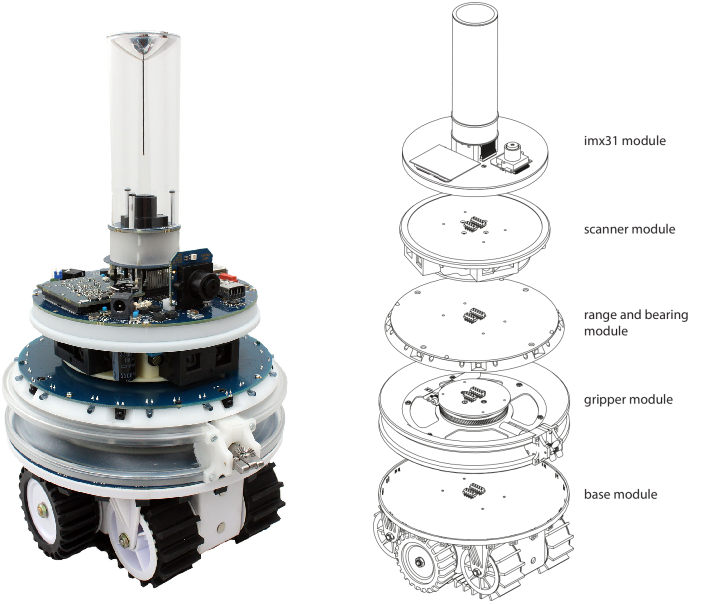
\includegraphics[width=.8\columnwidth]{introduction/marxbot}}
	\caption{Actual image and exploded CAD view of a marXbot.}
	\label{fig:marxbot}
\end{figure}

The target platform we choose for our project is the 
marXbot~\cite{bonani2010marxbot}, a research robot originally designed to study 
collective and swarm robotics. The main characteristic making the marXbot 
interesting for this project is its rotating laser scanner, which perceives 
distances and colours of the objects surrounding the robot.

The experiments are run in Enki~\cite{enki}, a high-performance open-source 
simulator for planar robots, which provides collision detection and limited 
physics support for robots evolving on a flat surface. Moreover, it can 
simulate groups of robots hundreds of times faster than real-time.

We explore the symbolic task of moving the robot to a specific pose with 
respect a certain object. While easy to accomplish when the exact poses of the 
robot and the goal object are known, it becomes non-trivial when only sensor 
data is available. In particular, the model must learn to extract 
characteristic features of the object surface that allow it to determine its 
pose. Furthermore, in our case the task is complicated by inherent ambiguities 
due to the symmetry of the chosen object. Sections~\ref{sec:controllers} and 
\ref{sec:task1} explore these aspects, how we dealt with them and the results 
we obtained from the experiments.

In Section~\ref{sec:task2} we instead attempt to generalise our model, so that 
the goal pose that it should reach can be arbitrary and provided as input.
